\newcommand{\exampleTwo} % Even
{
\begin{center}
\begin{tikzpicture}[shorten >=1pt,node distance=2cm,on grid,auto,scale=0.8,every node/.style={scale=0.8}]
    \node[state,initial,accepting,initial text=$Z$] (s0) {$s_0$};
    \node[state] (s1) [right=of s0] {$s_1$};
    \path[->]
        (s0)    edge [bend left=25] node {$S$}       (s1)
        (s1)    edge [bend left=25] node {$S$}       (s0)
    ;
\end{tikzpicture}
\end{center}
}
\newcommand{\forkJoinExample} % Even
{%
\begin{center}%
\begin{tikzpicture}[shorten >=1pt,node distance=4cm,on grid,auto,scale=1.0,every node/.style={scale=1.0}]
    \node[state,initial,accepting,initial text=$Seq$] (s0) {$s_0$};
    \node[state] (s1) [right=of s0] {$s_1$};
    \path[->]
        (s0)    edge [bend left=25] node {$Join$}       (s1)
        (s1)    edge [bend left=25] node {$Fork$}       (s0)
    ;
\end{tikzpicture}%
\end{center}%
}

\newcommand{\exampleOne}{\begin{center} % inc % 3
  \begin{tikzpicture}[shorten >=1pt,node distance=2cm,on grid,auto,scale=0.8,every node/.style={scale=0.8}]
      \node[state,initial,initial text=Z] (s0) {$s_0$};
      \node[state] (s1) [above right=0.25cm and 2cm of s0] {$s_1$};
      \node[state] (s2) [below right=0.25cm and 2cm of s1] {$s_2$};
      % \node[state,accepting] (s3) [right=of s2] {$s_3$};
      % \node[state] (s4) [right=of s3] {$s_4$};
      \path[->]
          (s0)    edge  [bend left=25]  node {$S$}      (s1)
          (s1)    edge   [bend left=25]            node {$S$}      (s2)
          (s2)    edge   [bend left=15]            node {$S$}         (s0)
          % (s0) edge [below] node {$*$} (s4)
      ;
  \end{tikzpicture}
  \end{center}%
  }

  \newcommand{\newworkflowWithTestersAndSelectors}
{%
\begin{figure}[h]
\centering
\tikzset{every picture/.style={line width=0.75pt}} %set default line width to 0.75pt        

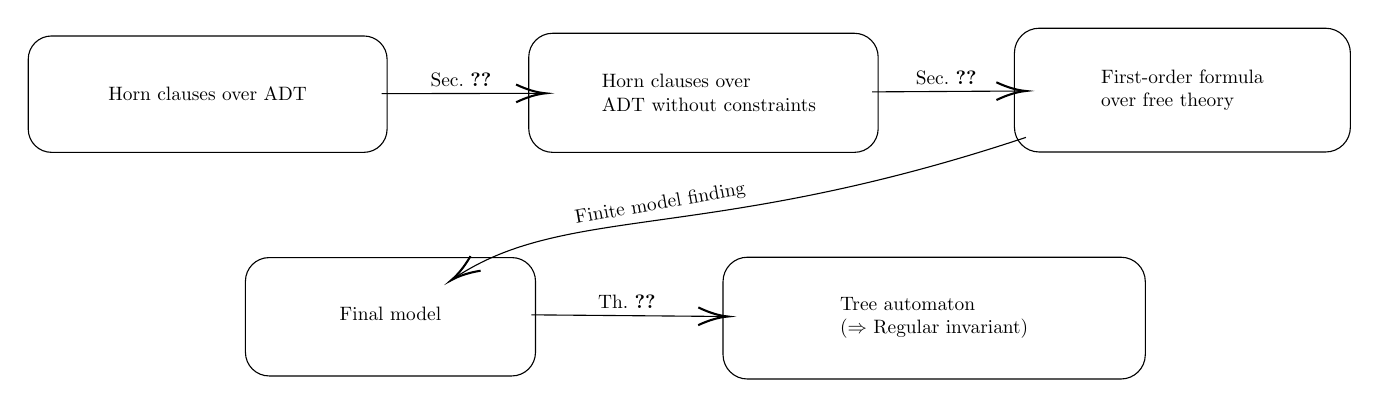
\begin{tikzpicture}[x=0.75pt,y=0.75pt,yscale=-1.3,xscale=1.3, every node/.style={scale=0.7}]
%uncomment if require: \path (0,300); %set diagram left start at 0, and has height of 300

%Rounded Rect [id:dp6178352482663523] 
\draw   (43.5,62.63) .. controls (43.5,57.86) and (47.36,54) .. (52.13,54) -- (167.88,54) .. controls (172.64,54) and (176.5,57.86) .. (176.5,62.63) -- (176.5,88.5) .. controls (176.5,93.26) and (172.64,97.13) .. (167.88,97.13) -- (52.13,97.13) .. controls (47.36,97.13) and (43.5,93.26) .. (43.5,88.5) -- cycle ;
%Rounded Rect [id:dp31517424205318467] 
\draw   (229,61.83) .. controls (229,56.95) and (232.95,53) .. (237.83,53) -- (349.68,53) .. controls (354.55,53) and (358.5,56.95) .. (358.5,61.83) -- (358.5,88.3) .. controls (358.5,93.17) and (354.55,97.13) .. (349.68,97.13) -- (237.83,97.13) .. controls (232.95,97.13) and (229,93.17) .. (229,88.3) -- cycle ;
%Rounded Rect [id:dp03467191946149972] 
\draw   (409,60.3) .. controls (409,55.23) and (413.11,51.13) .. (418.18,51.13) -- (524.33,51.13) .. controls (529.39,51.13) and (533.5,55.23) .. (533.5,60.3) -- (533.5,87.83) .. controls (533.5,92.89) and (529.39,97) .. (524.33,97) -- (418.18,97) .. controls (413.11,97) and (409,92.89) .. (409,87.83) -- cycle ;
%Rounded Rect [id:dp5801423669885661] 
\draw   (124,144.9) .. controls (124,140.05) and (127.93,136.13) .. (132.78,136.13) -- (222.73,136.13) .. controls (227.57,136.13) and (231.5,140.05) .. (231.5,144.9) -- (231.5,171.23) .. controls (231.5,176.07) and (227.57,180) .. (222.73,180) -- (132.78,180) .. controls (127.93,180) and (124,176.07) .. (124,171.23) -- cycle ;
%Rounded Rect [id:dp6969866775126601] 
\draw   (301,145.03) .. controls (301,140.04) and (305.04,136) .. (310.02,136) -- (448.48,136) .. controls (453.46,136) and (457.5,140.04) .. (457.5,145.03) -- (457.5,172.1) .. controls (457.5,177.08) and (453.46,181.13) .. (448.48,181.13) -- (310.02,181.13) .. controls (305.04,181.13) and (301,177.08) .. (301,172.1) -- cycle ;

\draw (471.25,74.06) node   [align=left] {First-order formula\\over free theory}; %без $\displaystyle \neq $,\\тестеров и селекторов};
% Text Node
\draw (110,75.56) node   [align=left] {Horn clauses over ADT};
% Text Node
\draw (295.75,75.06) node   [align=left] {Horn clauses over \\ ADT without constraints}; %$\displaystyle \neq $,\\тестеров и селекторов};
% Text Node
\draw (177.75,157) node   [align=left] {Final model};
% Text Node
\draw (379.25,158.56) node   [align=left] {Tree automaton\\($\displaystyle \Rightarrow $ Regular invariant)};

% % Text Node
% \draw (471.25,74.06) node   [align=left,execute at begin node=\setlength{\baselineskip}{1ex}] {CHCs over EUF\\without $\displaystyle \neq $, testers\\and selectors};
% % Text Node
% \draw (110,75.56) node   [align=left] {CHCs over ADTs};
% % Text Node
% \draw (295.75,75.06) node   [align=left,execute at begin node=\setlength{\baselineskip}{1ex}] {CHCs over ADTs\\without $\displaystyle \neq $, testers\\and selectors};
% % Text Node
% \draw (177.75,157) node   [align=left] {Finite model};
% % Text Node
% \draw (379.25,158.56) node   [align=left] {Tree tuples automata\\($\displaystyle \Rightarrow $Herbrand model)};
% Connection
\draw    (174.5,75.38) -- node[above] {Sec.~\ref{sec:fmf/totalCorrectness}} (233.25,75.25);
\draw [shift={(235.25,75.25)}, rotate = 539.8299999999999] [color={rgb, 255:red, 0; green, 0; blue, 0 }  ][line width=0.75]    (10.93,-3.29) .. controls (6.95,-1.4) and (3.31,-0.3) .. (0,0) .. controls (3.31,0.3) and (6.95,1.4) .. (10.93,3.29)   ;
% Connection
\draw    (356.25,74.72) -- node[above] {Sec.~\ref{sec:fmf/partialCorrectness}} (411.25,74.4) ;
\draw [shift={(413.25,74.39)}, rotate = 539.6700000000001] [color={rgb, 255:red, 0; green, 0; blue, 0 }  ][line width=0.75]    (10.93,-3.29) .. controls (6.95,-1.4) and (3.31,-0.3) .. (0,0) .. controls (3.31,0.3) and (6.95,1.4) .. (10.93,3.29)   ;
% Connection
\draw    (413.25,91.58) .. controls (295.23,130.94) and (243.1,115.96) .. node[above,rotate=10] {Finite model finding} (201.55,143.65) ;
\draw [shift={(200.29,144.5)}, rotate = 325.36] [color={rgb, 255:red, 0; green, 0; blue, 0 }  ][line width=0.75]    (10.93,-3.29) .. controls (6.95,-1.4) and (3.31,-0.3) .. (0,0) .. controls (3.31,0.3) and (6.95,1.4) .. (10.93,3.29)   ;
% Connection
\draw    (230,157.35) -- node[above] {Th.~\ref{thm:finite-to-automaton}} (300.75,157.95) ;
\draw [shift={(302.75,157.97)}, rotate = 180.44] [color={rgb, 255:red, 0; green, 0; blue, 0 }  ][line width=0.75]    (10.93,-3.29) .. controls (6.95,-1.4) and (3.31,-0.3) .. (0,0) .. controls (3.31,0.3) and (6.95,1.4) .. (10.93,3.29)   ;
\end{tikzpicture}
\caption{Regular invariant inference method for a Horn clause system over ADT}
\label{fig:newworkflow-with-testers-selectors}
\end{figure}%
}

\newcommand{\exampleCostruction}
{
\begin{center}
\begin{tikzpicture}[shorten >=1pt,node distance=2cm,on grid,auto,scale=0.8,every node/.style={scale=0.8}]
    \node[state,initial,accepting,initial text=$Z$] (s0) {$0$};
    \node[state] (s1) [right=of s0] {$1$};
    \path[->]
        (s0)    edge [bend left=25] node {$S$}       (s1)
        (s1)    edge [bend left=25] node {$S$}       (s0)
    ;
\end{tikzpicture}
\end{center}
}

\newcommand{\defPumpLemmaElem}{%
\begin{restatable}[Pumping Lemma for \elemclass{}]{lemma}{pumplemmaelem}\label{lemm:pump-elem}
Let $\formallang{}$ be an elementary language of $n$-tuples. Then, there exists a constant $K > 0$ satisfying:
\begin{itemize}
    \item for every $n$-tuples of ground terms $\tuple{g_1,\ldots,g_n} \in \formallang{}$,
    \item for any $i$ such that $\height{g_i} > K$,
    \item for all infinite sorts $\sigma \in \sorts$ and
    \item for all paths $p$ with a length greater than $K$,
    \item there exist finite sets of paths $P_j$ such that $p \in P_i$,
    \item for all $p_1, p_2 \in \bigcup_j P_j$ it is true that $p_1(g) = p_2(g)$,
    \item and there is $N \geq 0$, such that
    \item for all $t$ of sort $\sigma$ with $\height{t} > N$ it holds that:
\end{itemize}
$$\tuple{g_1[P_1\leftarrow t],\ldots,g_i[P_i\leftarrow t],\ldots,g_n[P_n\leftarrow t]} \in \formallang{}.$$
\end{restatable}
}

\newcommand{\defPumpLemmaSizeElem}{%
\begin{restatable}[Pumping Lemma for \sizeelemclass{}]{lemma}{pumplemmasizeelem}\label{lemm:pump-sizeelem}
Let the ADT signature be expanding and let $\formallang{}$ be an elementary language of $n$-tuples with size constraints. Then, there exists a constant $K > 0$ satisfying:
\begin{itemize}
\item for every $n$-tuple of ground terms $\tuple{g_1,\ldots,g_n} \in \formallang{}$,
\item for any $i$, such that $\height{g_i} > K$,
\item for all infinite sorts $\sigma \in \sorts$, and
\item for all paths $p \in \leafpos{\sigma}{g_i}$ with length greater than $K$,
\item there exists an infinite linear set $T \subseteq \sizesOfSort{\sigma}$, such that
\item for all terms $t$ of sort $\sigma$ with sizes $\sizename{}(t) \in T$,
\item there exist sequences of paths $P_j$, with no path in them being a suffix of path $p$,
\item and sequences of terms $U_j$, such that
\end{itemize}
$$\tuple{g_1[P_1\!\leftarrow\! U_1],\ldots,g_i[p \!\leftarrow\! t, P_i \!\leftarrow\! U_i],\ldots,g_n[P_n \!\leftarrow\! U_n]} \in \formallang{}.$$
\end{restatable}
}

\newcommand{\invariantreprclasses}[1]
{
\begin{figure}[t]
\tikzset{every picture/.style={line width=0.75pt}} %set default line width to 0.75pt       
\centering
\begin{tikzpicture}[shorten >=1pt,auto,node distance=15mm,scale=1.0,every state/.style={scale=1.0,minimum width=26mm}]
    \node[state] (regElem) {\regelemclass{}};
    \node (regElemL) [left=of regElem] {};
    \node (regElemR) [right=of regElem] {};
    \node[state] (elem) [below=of regElemL] {\elemclass{}};
    \node[state] (reg) [below=of regElemR] {\regclass{}};
    \node[state] (sizeelem) [left=of regElemL] {\sizeelemclass{}};
    \node[state] (syncFlat) [right=of regElemR] {\syncRegFlatClass{}};
    \node[state] (syncFull) [above=of syncFlat] {\syncRegFullClass{}};
    \path[->]
        (elem)    edge node {\exLt}       (sizeelem)
        (elem)    edge node {\exEvenLeft\footnotemark}       (regElem)
        (reg)    edge node {\exLR\footnotemark}       (regElem)
        (reg)    edge node {\exLt\footnotemark}       (syncFlat)
        (syncFlat)    edge node {\exNode\footnotemark}       (syncFull)
    ;
\end{tikzpicture}
\caption{Inclusion relations between classes of inductive invariants over ADTs.}%Связи включения между классами индуктивных инвариантов над АТД. 
#1
\end{figure}
\footnotetext[1]{$\exEvenLeft{} \in \regclass{} \setminus \sizeelemclass{}$ (Theorem~\ref{thm:exEvenLeft})}
\footnotetext[2]{$\exLR{}\in\elemclass{} \setminus \syncRegFullClass{}$ (Lemma~\ref{lemm:lr-not-in-reg-full})}
\footnotetext[3]{$\exLt\in\syncRegFlatClass{}\setminus\regclass{}$ (Theorem~\ref{thm:exLt})}
\footnotetext[4]{$\exNode\in\syncRegFullClass{}\setminus\syncRegFlatClass{}$ (Lemma~\ref{lemm:node-not-in-reg-flat})}
}

\newcommand{\toolplotOne}{
\pgfplotstableread[col sep = comma]{Dissertation/images/experiments1.csv}\all
\begin{figure}[t!]
\begin{center}
\begin{tikzpicture}[scale=1.2]
\begin{axis}[xmode=log, ymode=log, legend pos= north west, xlabel={Runtime of \ringen{\cvc{}}, ms}, xlabel style = {align=center,font=\footnotesize}, ylabel style = {align=center,font=\footnotesize}, ylabel={Runtime of {\color{red}\racer{}}, {\color{blue}\eldarica{}},\\{\color{brown}\cvcind{}} and {\color{cyan}\verimap{}}, ms}]
% \begin{axis}[xmode=log, ymode=log, legend pos= north west, xlabel={ Regular model construction by \theringen{}}, ylabel style = {align=center}, ylabel={Elementary model construction by \\{\color{red}\textsc{Spacer}}, {\color{blue}\eldarica{}} and {\color{brown}\cvcind{}}}]
    \addplot[dashed,no marks,very thin] coordinates {(10,10) (600000,600000)};
    \addplot [dashed, no marks, thin] coordinates {(10,10) (600000,600000)};
    \addplot [dashed, no marks, thin] coordinates {(10,300000) (300000,300000)};
    \addplot [dashed, no marks, thin] coordinates {(300000, 10) (300000,300000)};
    \addplot [dashed, no marks, thin] coordinates {(10, 600000) (600000,600000)};
    \addplot [dashed, no marks, thin] coordinates {(600000, 10) (600000,600000)};

    \addplot  [only marks,  mark=triangle, color=blue, mark size=3pt] table [x={CVC4Finite}, y={Eldarica}] {\all};
    \addplot  [only marks,  mark=o, color=red,  mark size=3pt] table [x={CVC4Finite}, y={Z3}] {\all};
    \addplot  [only marks,  mark=x, color=brown, mark size=3pt] table [x={CVC4Finite}, y={CVC4Ind}] {\all};
    \addplot  [only marks,  mark=square, color=cyan, mark size=3pt] table [x={CVC4Finite}, y={VeriMAP-iddt}] {\all};
\end{axis}

\end{tikzpicture}
    \caption{ Performance comparison. Each point on the plot represents a pair of runtimes.} %Сравнение производительности инструментов. Каждая точка на графике представляет пару длительностей выполнения.
\label{fig:toolplotOne}
\end{center}
\end{figure}
}

\newcommand{\fmfModelSizes}{
\pgfplotstableread[col sep = comma]{Dissertation/images/cards.csv}\all
\begin{figure}[ht!]
\begin{center}

\begin{tikzpicture}[scale=1.0]
  \begin{axis}[
  xlabel={Размер модели},
  ylabel={Число моделей},
  ybar,
  xtick distance=1,
  ytick distance=1,
    ]
    \addplot+ table {\all};
  \end{axis}
\end{tikzpicture}
\caption{Размеры конечных моделей, построенных инструментом \cvc{}~--- сторонним решателем, вызываемым инструментом \theringen{}. Размер модели (на оси абсцисс) считается как \emph{сумма} мощностей всех сортов.}
\label{fig:cardinalities}
\end{center}
\end{figure}
}

\newcommand{\toolplotsatOne}{
\pgfplotstableread[col sep = comma]{Dissertation/images/expsat1.csv}\allsat
\begin{figure}[t!]
\begin{center}
\begin{tikzpicture}[scale=1.2]
\begin{axis}[xmode=log, ymode=log, legend pos= north west, xlabel={Время построения регулярных инвариантов\\при помощи \theringen{}, сек.}, xlabel style = {align=center,font=\footnotesize}, ylabel style = {align=center,font=\footnotesize}, ylabel={Время построения элементарных\\инвариантов при помощи {\color{red}\zprover{}}, {\color{blue}\eldarica{}},\\{\color{brown}\cvcind{}} и {\color{cyan}\verimap{}}, сек.}]
    \addplot[dashed,no marks,very thin] coordinates {(10,10) (600000,600000)};
    \addplot [dashed, no marks, thin] coordinates {(10,10) (600000,600000)};
    \addplot [dashed, no marks, thin] coordinates {(10,300000) (300000,300000)};
    \addplot [dashed, no marks, thin] coordinates {(300000, 10) (300000,300000)};
    \addplot [dashed, no marks, thin] coordinates {(10, 600000) (600000,600000)};
    \addplot [dashed, no marks, thin] coordinates {(600000, 10) (600000,600000)};

    \addplot  [only marks,  mark=triangle, color=blue, mark size=3pt] table [x={CVC4Finite}, y={Eldarica}] {\allsat};
    \addplot  [only marks,  mark=o, color=red,  mark size=3pt] table [x={CVC4Finite}, y={Z3}] {\allsat};
    \addplot  [only marks,  mark=x, color=brown, mark size=3pt] table [x={CVC4Finite}, y={CVC4Ind}] {\allsat};
    \addplot  [only marks,  mark=square, color=cyan, mark size=3pt] table [x={CVC4Finite}, y={VeriMAP-iddt}] {\allsat};
\end{axis}
\end{tikzpicture}
    \caption{Сравнение производительности инструментов \emph{только на результатах \foreignlanguage{english}{<<SAT>>}}. Тест включается в этот график, если хотя бы один из инструментов обнаружил инвариант.}
\label{fig:toolplotsat}
\end{center}
\end{figure}
}

\newcommand{\toolplotTwo}[2]{%
% #1 is backend solver name
% #2 is a .csv file name
\pgfplotstableread[col sep = comma]{#2}\toolplotcsv
\begin{subfigure}[t]{0.47\textwidth}
\begin{center}
\begin{tikzpicture}[scale=.93]
\begin{axis}[xmode=log, ymode=log, legend pos= north west, xlabel={\ringenCICI{#1}, ms}, ylabel style = {align=center}, ylabel={{\color{red}\racer{}} and {\color{blue}\ringen{#1}}, ms}]
    \addplot[dashed,no marks,very thin] coordinates {(10,10) (1200000,1200000)};
    \addplot [dashed, no marks, thin] coordinates {(10,10) (1200000,1200000)};
    \addplot [dashed, no marks, thin] coordinates {(10,600000) (600000,600000)};
    \addplot [dashed, no marks, thin] coordinates {(600000, 10) (600000,600000)};
    \addplot [dashed, no marks, thin] coordinates {(10, 1200000) (1200000,1200000)};
    \addplot [dashed, no marks, thin] coordinates {(1200000, 10) (1200000,1200000)};
    
    % one second
    \addplot [no marks, thin] coordinates {(1000, 10) (1000,1000)};
    \addplot [no marks, thin] coordinates {(10, 1000) (1000,1000)};

    \addplot  [only marks,  mark=o, color=red,  mark size=3pt] table [x={Collab}, y={Z3}] {\toolplotcsv};
    \addplot  [only marks,  mark=triangle, color=blue, mark size=3pt] table [x={Collab}, y={RInGen}] {\toolplotcsv};
\end{axis}
\end{tikzpicture}
\end{center}
\end{subfigure}
}

\newcommand{\PattternAutomata}{
    \begin{figure*}[h]
    \centering
    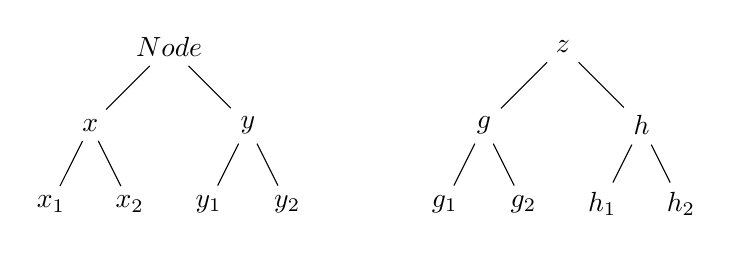
\begin{tikzpicture}[node distance=2cm,remember picture]
    
    \node (A) at (1,0) {$Node$};
    \node (B) at (0,-1){$x$};
    \node (B1) at (-0.5,-2){$x_1$};
    \node (B2) at (0.5,-2){$x_2$};
    
    \node (C) at (2,-1){$y$};
    \node (C1) at (1.5,-2){$y_1$};
    \node (C2) at (2.5,-2){$y_2$};
    
    \draw[-] (A) -- (B);
    \draw[-] (A) -- (C);
    \draw[-] (B) -- (B1);
    \draw[-] (B) -- (B2);
    
    \draw[-] (C) -- (C1);
    \draw[-] (C) -- (C2);
    
    \node (D) at (6,0) {$z$};
    \node (E) at (5,-1){$g$};
    \node (F) at (7,-1){$h$};
    \node (E1) at (4.5,-2){$g_1$};
    \node (E2) at (5.5,-2){$g_2$};
    
    \node (F1) at (6.5,-2){$h_1$};
    \node (F2) at (7.5,-2){$h_2$};
    
    \draw[-] (D) -- (E);
    \draw[-] (D) -- (F);
    \draw[-] (E) -- (E1);
    \draw[-] (E) -- (E2);
    \draw[-] (F) -- (F1);
    \draw[-] (F) -- (F2);
    
    \end{tikzpicture}
    \label{fig:ref-stdSync}
    \end{figure*}
    }

\newcommand{\ltAutomaton}{
    \begin{figure}[h]
    \centering
    \begin{tikzpicture}[scale=1]
 
    \node [state] {$q_0$};
    \node (q0) [state,
    initial,
    initial left,
    initial distance=0.5cm,
    initial text=$\tuple{\bot, \bot}$
] {$q_0$};
    \node (q1) [state, accepting] at (3,1) {$q_1$};
    \node (q2) [state] at (3,-1) {$q_2$};

    \path [-stealth, thick]
        (q0) edge [bend left] node [above] {$\tuple{\bot, Z}$}   (q1)
        (q0) edge [bend right] node [below] {$\tuple{Z, \bot}$}   (q2)
        (q1) edge [loop right]  node {*}()
        (q2) edge [loop right]  node {*}();

    \end{tikzpicture}
    %\caption{Синхронный древовидный автомат для предикатного символа $lt$}\label{fig:ltAutomata}
    \end{figure}
}